% 等压过程
% 等压过程|体积|压强|状态方程|做功

\pentry{理想气体状态方程\upref{PVnRT}}

等压过程的特征是系统的压强保持不变,即$p $为常量,$\mathrm dp =0$.设想气缸连续地与一系列有微小温度差的恒温热源相接触,同时活塞上所加的外力保持不变.那么接触产生什么效果呢?就是将有微小的热量传给气体,使气体温度稍微升高,气体对活塞的压强也随之较外界所施的压强增加一微量,于是稍微推动活塞对外做功.由于体积的膨胀,压强降低,从而保证气体在内、外压强的量值保持不变的情况下进行膨胀.所以这一准静态过程是一个\textbf{等压过程(isobaric process)},如\autoref{EqPre_fig1}所示.
\begin{figure}[ht]
\centering
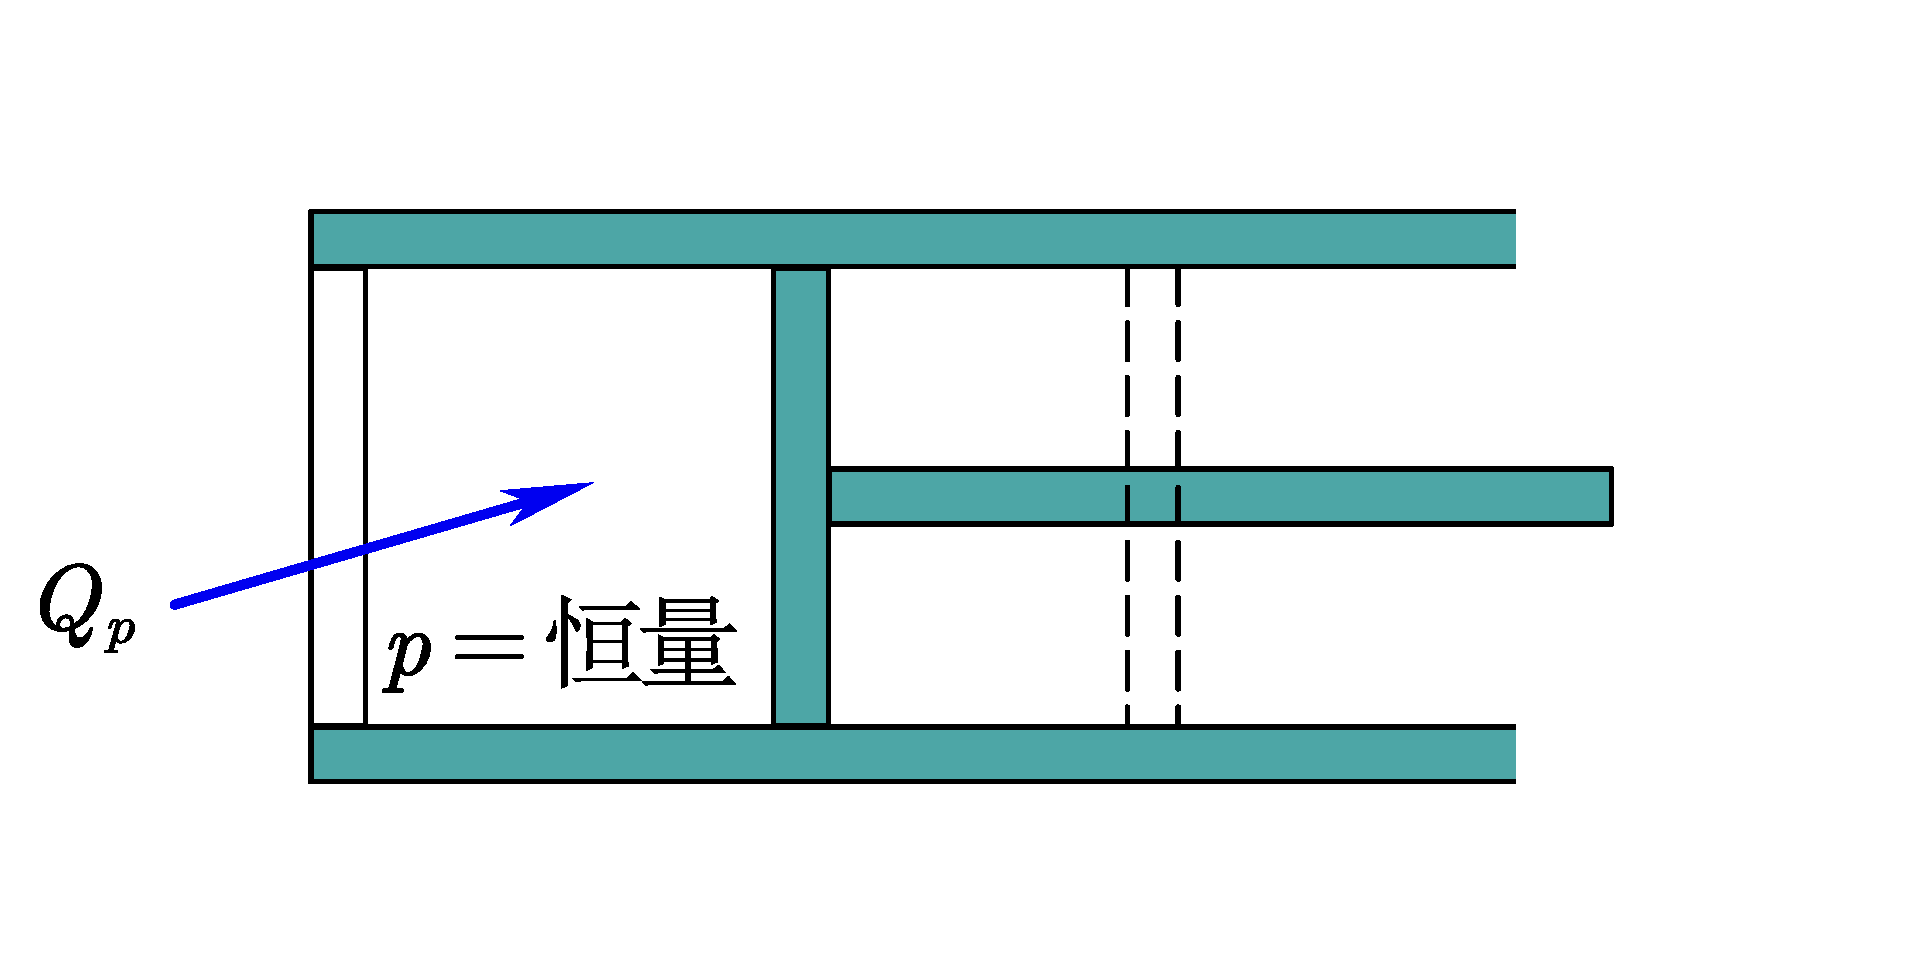
\includegraphics[width=8cm]{./figures/EqPre_1.pdf}
\caption{气体的等压过程} \label{EqPre_fig1}
\end{figure}
现在我们来计算气体的体积增加$\mathrm d V $时所做的功$\delta W$.根据理想气体状态方程,如果气体的体积从$V $增加到$V+\mathrm dV$,温度从$T $增加到$T+\mathrm dT$,那么气体所做的功
\begin{equation}
\delta W=p \mathrm{d} V=\frac{m}{M} R \mathrm{d} T
\end{equation}
\begin{figure}[ht]
\centering
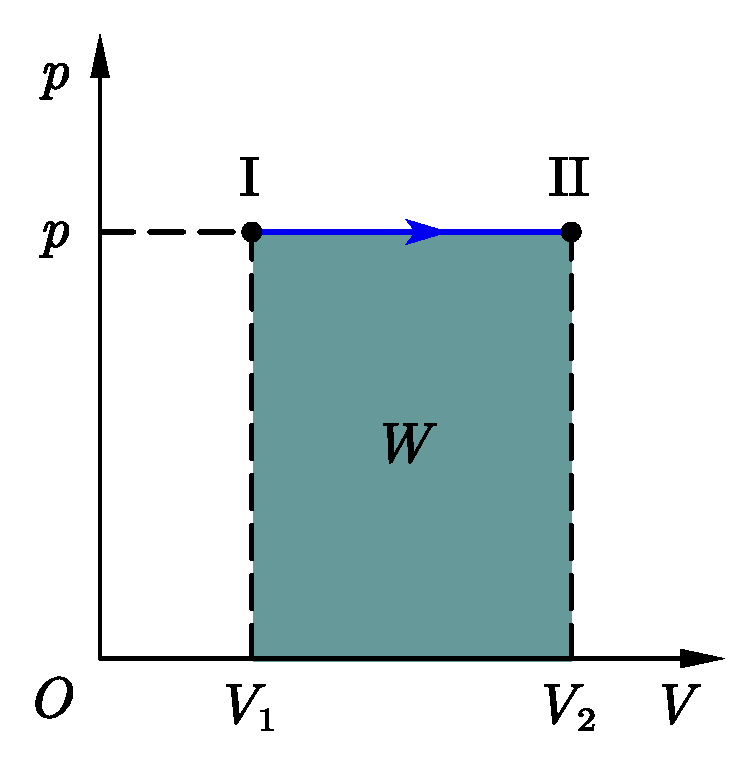
\includegraphics[width=5cm]{./figures/EqPre_2.pdf}
\caption{等压过程中功的计算} \label{EqPre_fig2}
\end{figure}
根据热力学第一定律,系统吸收的热量为
\begin{equation}
\delta Q_{p}=\mathrm{d} E+\frac{m}{M} R \mathrm{d} T
\end{equation}
式中,下角标$p $表示压强不变.当气体从状态$\mathrm I(p, V_1, T_1)$等压地变为状态$\mathrm{II}(p, V_2,T_2)$时,气体对外做功为
\begin{equation}
W=\int_{V_{1}}^{V_{2}} p \mathrm{d} V=p\left(V_{2}-V_{1}\right)
\end{equation}
或写成
\begin{equation}
W=\int_{T_{1}}^{T_{2}} \frac{m}{M} R \mathrm{d} T=\frac{m}{M} R\left(T_{2}-T_{1}\right)
\end{equation}
所以,整个过程中传递的热量为
\begin{equation}
Q_{p}=E_{2}-E_{1}+\frac{m}{M} R\left(T_{2}-T_{1}\right)
\end{equation}

气体在等压膨胀过程中,所吸收的热量的一部分用来增加内能,另一部分用于气体对外做功;气体在等压压缩过程中,外界对气体做功,同时内能减小,其和等于放出的热量.

我们把$1\mathrm{mol}$气体在压强不变的条件下,温度改变$1\mathrm K$所需要的热量叫做气体的\textbf{摩尔定压热容(molar heat capacity at constant pressure)},用$C_{p,m}$表示,即
\begin{equation}
C_{p, {m}}=\frac{\delta Q_{p}}{\frac{m}{M} \mathrm{d} T}
\end{equation}
根据这个定义可得
\begin{equation}
\delta Q_{p}=\frac{m}{M} C_{p, {m}} \mathrm{d} T
\end{equation}
又因
\begin{equation}
E_{2}-E_{1}=\frac{m}{M} C_{V, \mathrm{m}}\left(T_{2}-T_{1}\right)
\end{equation}
我们得到
\begin{equation} \label{EqPre_eq1}
C_{p, m}=C_{V, m}+R
\end{equation}

\autoref{EqPre_eq1}叫做\textbf{迈耶(J. R. Meyer)公式}.它的意义是,$1\; \rm mol$理想气体温度升高$1\rm K$时,在等压过程中比在等体过程中要多吸收$8. 31\rm J $的热量.这部分热量去哪了呢?当然是转化为对外所做的膨胀功.由此可见,普适气体常量$R$等于$1\;\rm mol$理想气体在等压过程中温度升高$1\rm K$对外所做的功.因$C_{v, m}=iR/2$,从\autoref{EqPre_eq1}可知
\begin{equation}
C_{p, {m}}=\frac{i}{2} R+R=\frac{i+2}{2} R
\end{equation}

摩尔定压热容$C_{p,m}$与摩尔定容热容$C_{V,m}$之比,用$\gamma$表示,叫做\textbf{[摩尔]热容比(ratio of [molar] heat capacity)}或\textbf{绝热指数},于是
\begin{equation} \label{EqPre_eq2}
\gamma=\frac{C_{p, \mathrm{m}}}{C_{V, \mathrm{m}}}=\frac{i+2}{i}
\end{equation}

根据\autoref{EqPre_eq2}不难算出:对于单原子分子气体,$\gamma=5/3\approx 1.67$;双原子刚性分子气体$\gamma=1.40$;多原子刚性分子气体$\gamma\approx 1. 33 $.它们也都只与气体分子的自由度有关,而与气体温度无关.

无论是定压热容,还是定容热容,它们的共同特点是体现了使物体温度发生变化的难易程度,热容大的物体同样升高$1\rm K$,所需要的热量也多,这说明温度不易变化,所以物体的热容是其\textbf{热惯性}的量度.

我们来看几个例题加深一下对内容的理解.

\begin{example}{温度计}
用作测温的温度计,为了能和被测物体迅速达到热平衡,它的热容必须很小.
\end{example}

\begin{example}{氮气加热}
一气缸中贮有氮气,质量为$1.25\rm kg$,在标准大气压下缓慢地加热,使温度升高$1\mathrm K$.试求气体膨胀时所做的功$W$、气体内能的增量$\Delta E$以及气体所吸收的热量$Q_p$.(活塞的质量以及它与气缸壁的摩擦均可略去).

因过程是等压的,所以
\begin{equation}
W=\frac{m}{M} R \Delta T=\frac{1.25}{0.028} \times 8.31 \times 1 \mathrm{J}=371 \mathrm{J}
\end{equation}
而因为氮气的$i=5$,所以
\begin{equation}
C_{V, {m}}=\frac{i}{2} R=20.8 \mathrm{J} /(\mathrm{mol} \cdot \mathrm{K})
\end{equation}
于是
\begin{equation}
\Delta E=\frac{m}{M} C_{V, {m}} \Delta T=\frac{1.25}{0.028} \times 20.8 \times 1 \mathrm{J}=929 \mathrm{J}
\end{equation}
所以,气体在这一过程中所吸收的热量为
\begin{equation}
Q_{p}=E_{2}-E_{1}+W=1300 \mathrm{J}
\end{equation}
\end{example}   